%%~~~~~~~~~~~~~~~~~~~~~~~~~~~~~~~~~~~~~~~~~~~~~~~~~~~
\frame{
\frametitle{GUI: Programmaufbau}
	\begin{block}{Anforderungen}
		\begin{itemize}
			\item Basisklasse GUI enthält mögliche Designelemente für einzelne Abschnitte der APP
			\item Seiten erben von Basisklasse und implementieren eigene Funktionalität
		\end{itemize}
	\end{block}
}

\frame{
\frametitle{Gui: Klassendiagramm}
	\begin{center}
			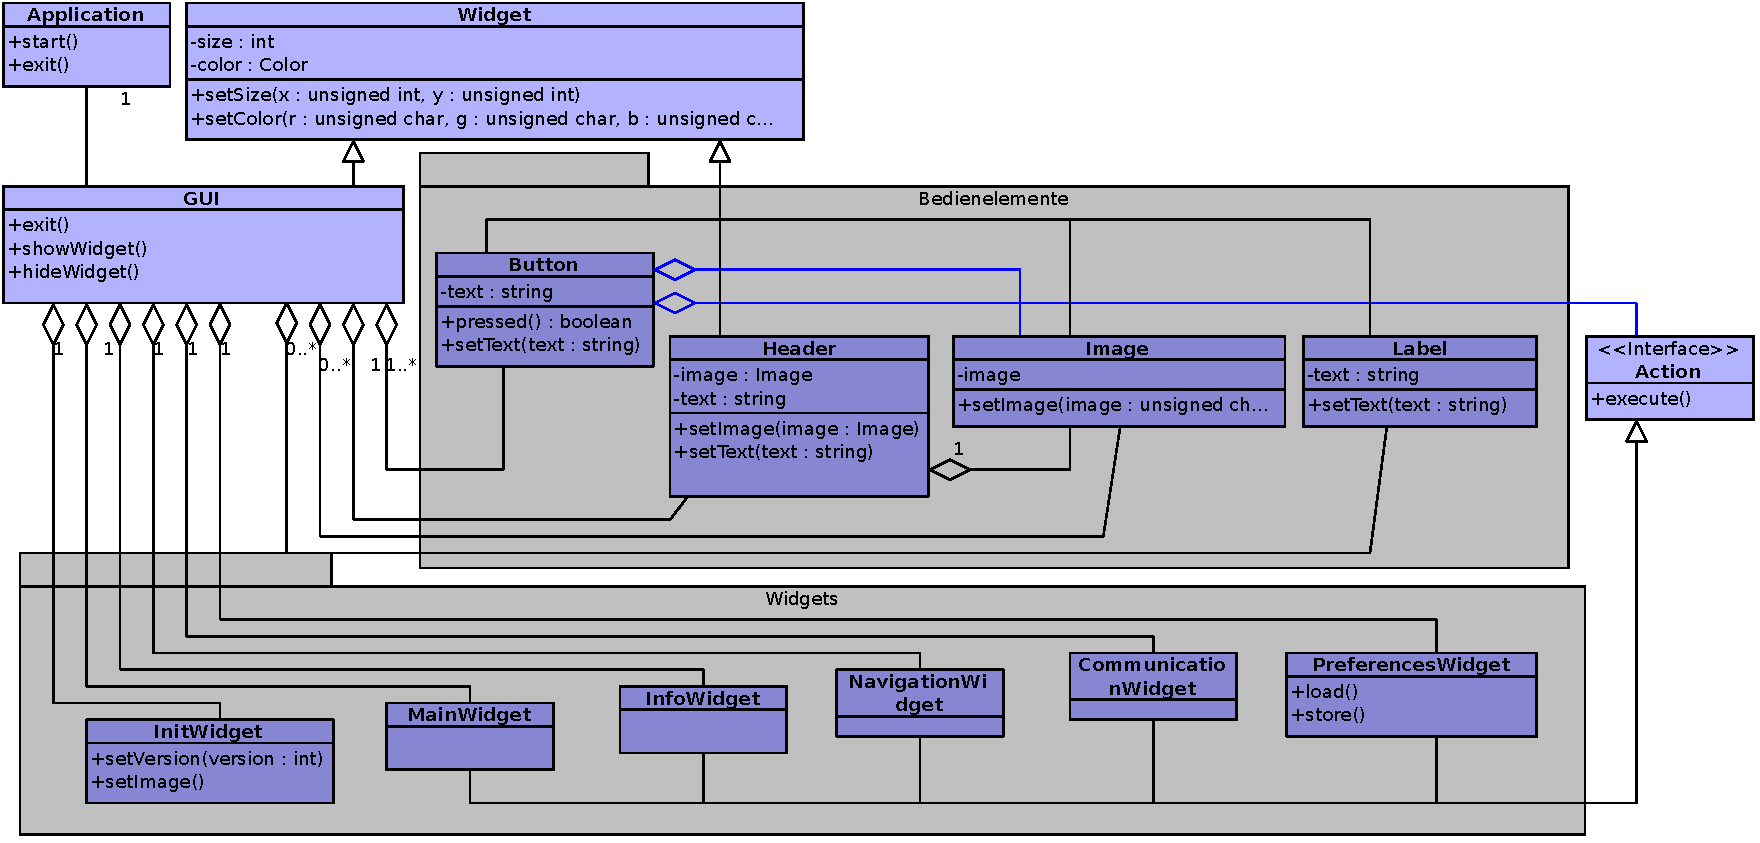
\includegraphics[width=0.9\textwidth]{../grafiken/GUI_Class.pdf}
	\end{center}
}


\frame{
\frametitle{Menüwechsel}
	\begin{block}{Zustandsmaschine}
		\begin{itemize}
			\item \textbf{Menüpunkte} werden als \textbf{Zustand} gesehen
			\item zusätzliche Zustände für \textbf{Start und Beenden} der Application
			\item Zustände können wiederum Unter-Zustände besitzen
		\end{itemize}
		\begin{center}
			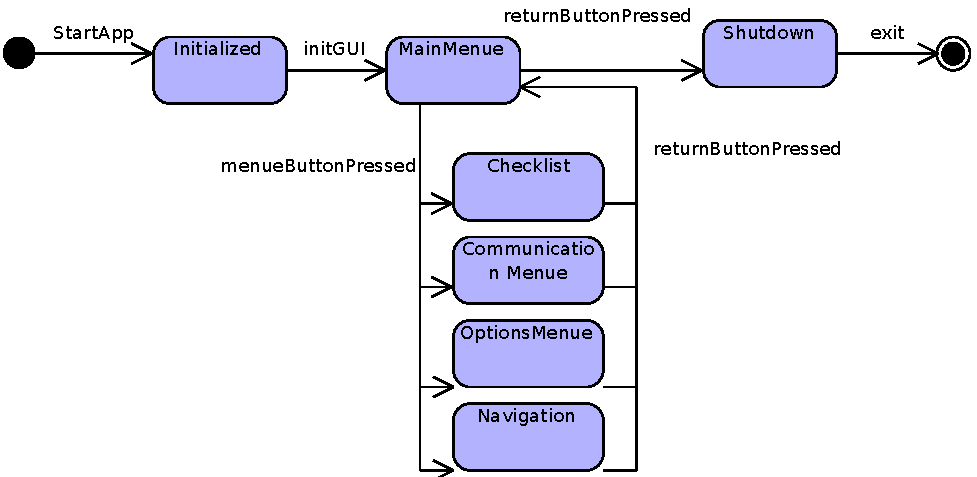
\includegraphics[width=0.65\textwidth]{../grafiken/MenueStates.pdf}
		\end{center}
	\end{block}
}
